\newcommand\version{v1}
\problemname{Vänner}
$N$ vänner spelar ett spel. Spelet spelas på en rad av $L$ rutor numrerade från $0$ till $L - 1$, där rutorna $i$ och $i+1$ är bredvid varandra. Som mest en av vänner kan stå på en ruta vid någon tidpunkt. I varje steg av spelet hoppar en av vännerna från sin nuvarande ruta till en tom ruta.

Vid någon tidpunkt i spelet är en spelares $poäng$ längden av det längsta sammanhängande segmentet av spelare personen är en del av. Det innebär att om en spelare står på position $x$ och det står andra spelare på positionerna $a, a+1, ..., x-1, x, x+1, ..., b-1, b$ så har spelaren poängen $b - a + 1$.

Den totala poängen är summan av alla spelares poäng. Vid olika tidpunkter i spelet undrar vännerna vad deras nuvarande totala poäng är.


\section*{Exempel}
Antag att det är $N = 3$ vänner som spelar på en spelplan av längd $L = 7$. I början befinner de sig på positionerna
$1, 3, 4$. Poängen för spelaren på position $1$ är bara $1$ eftersom inga vänner är direkt till vänster eller höger.
Spelarna på positionerna $3$ och $4$ utgör ett segment av längd $2$, så båda har $2$ poäng. Den totala poängen i den här tidpunkten är $1 + 2 + 2 = 5$.

Första hoppet är från position $4$ till $2$ vilket ger de nya positionerna $1, 2, 3$. Här är utgör alla spelare tillsammans
ett segment av längd $3$, så alla spelare har $3$ poäng vilket ger den totala poängen $9$.

Det andra och sista hoppet är från $3$ till $0$, vilket ger positionerna $0, 1, 2$. All spelare utgör
fortfarande ett segment av längd $3$, så den totala poängen är fortfarande $9$.

\begin{figure}[h!]
  \centering
  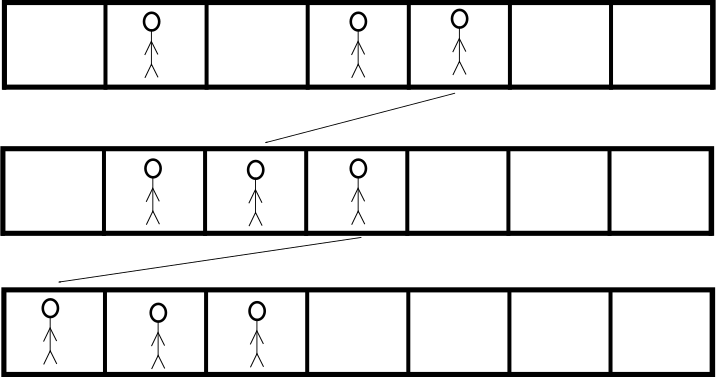
\includegraphics[width=0.8\textwidth]{sample.png}
  \caption{Illustration av exemplet}
\end{figure}

\section*{Uppgift}
Du kommer att få alla hopp som görs i spelet. Vid några tidpunkter kommer vännerna att fråga vad den totala poängen är. Din uppgift är 
att implementera funktionerna \texttt{init(N, L, P)}, \texttt{jump(A, B)}, and \texttt{score()}:
\begin{itemize}
  \item \texttt{init(N, L, P)} - den här funktionen kommer at anropas precis en gång av domaren vid spelets början.
  \begin{itemize}
    \item \texttt{N}: antalet spelare.
    \item \texttt{L}: antalet rutor i spelet.
    \item \texttt{P}: en array med $N$ element. \texttt{P[i]} ($0 \le i < N$) anger startpositionen för den $i$:te spelaren.
    \item Funktionen ska inte returnera något.
  \end{itemize}

  \item \texttt{jump(A, B)} - den här funktionen anropas varje gång en spelare gör ett hopp, i den ordning som hoppen görs.
  \begin{itemize}
    \item \texttt{A}: positionen som spelaren hoppar från ($0 \le A < L$). Det kommer alltid att finnas en spelare på den positionen när hoppet görs.
    \item \texttt{B}: positionen som spelaren hoppar till ($0 \le B < L$). Det kommer aldrig att finnas en spelare på den positionen när hoppet görs.
    \item Funktionen ska inte returnera något.
  \end{itemize}

  \item \texttt{score()} - den här funktionen anropas när vännerna vill veta sin totala poäng.
  \begin{itemize}
    \item Funktionen ska returnera den totala poängen.
  \end{itemize}

\end{itemize}

\section*{Delpoäng}
Problemet består av flera grupper av testfall. Varje grupp ger ett visst antal poäng och för att klara det måste du klara alla testfall i gruppen.

Låt $J$ vara antalet anrop till \texttt{jump} och $S$ vara antalet anrop till \texttt{score}.

\begin{tabular}{|l|l|l|}
  \hline
  \textbf{Grupp} & \textbf{Poäng} & \textbf{Gränser} \\ \hline
  1 & 9 & $1 \le N, L \le 1\,000$,  $S + J \le 2\,000$ \\ \hline
  2 & 17 & $1 \le N, L \le 100\,000$, $J = 0$, $S = 1$ \\ \hline
  3 & 14 & $1 \le N \le 100\,000$, $1 \le N \le 10^9$, $J = 0$, $S = 1$ \\ \hline
  4 & 38 & $1 \le N, L \le 100\,000$, $S + J \le 200\,000$ \\ \hline
  5 & 22 & $1 \le N \le 100\,000$, $1 \le N \le 10^9$, $S + J \le 200\,000$ \\ \hline
\end{tabular}

\section*{Input format}
Exempeldomaren läser indata i följande format:

\begin{itemize}
  \item rad $1$: \texttt{N L Q}
  \item rad $2$: \texttt{P[0] P[1] .. P[N - 1]}
  \item raderna $3$ till $3 + Q - 1$: varje rad representerar ett hopp eller en fråga om poängen.
    Om raden är \texttt{0 A B} så görs ett hopp från $A$ till $B$. Om raden är \texttt{1} så frågar vännerna om den totala poängen.
\end{itemize}

\section*{Output format}
Varje gång den totala poängen efterfrågas skriver domaren en rad med returnvärdet från \texttt{score()}.
